\documentclass[a4paper,12pt]{article}

% Font configuration for Times New Roman
\usepackage{mathptmx}
\usepackage[T1]{fontenc}

% Page geometry settings (25mm top/bottom, 20mm left/right)
\usepackage[top=25mm, bottom=25mm, left=20mm, right=20mm]{geometry}

% Remove page numbers, headers, and footers
\pagestyle{empty}

% Optional packages for tables and graphics
\usepackage{graphicx}
\usepackage{booktabs}
\usepackage[natbibapa]{apacite}

% Custom command for run-in headings
\newcommand{\heading}[1]{%
  \noindent\textbf{#1}%
}

\newcommand{\kommentti}[1]{{\bf[#1]}}

\setlength{\parskip}{1em}
\setlength{\parindent}{0em}

\begin{document}

% Top Matter
\begin{center}
    {\fontsize{13.4pt}{12pt}\selectfont
    \textbf{You Should Plug Your Telemed Ultrasound to Mains Power}\par}
    % \vspace{1em}
    {\fontsize{12pt}{10pt}\selectfont
    Pertti Palo\par
    \vspace{0.25em}
    University of Alberta, Edmonton, Alberta, Canada
    \vspace{0.25em}
    pertti.palo@taurlin.org\par
    \vspace{-0.75em}
    }
\end{center}

\heading{Introduction.}
Ultrasound has been used for speech studies for decades
\citep{ShawkerSonies-UltrasoundBiofeedbackSpeech-1985,Gick-UseUltrasoundLinguistic-2002,Stone-GuideAnalyzingTongue-2005}
In recent years Telemed micro ultrasound devices have become something of a
norm. While the manual says to use mains power (connect the ultrasound device's
power source to a wall socket) it does not say why, and the device will work
with just power from the USB-connection to a computer.
We discovered by accident why this recommendation exists: When running on USB
power the ultrasound device will raise imaging power by steps during each
recording. According to Telemed, this is done to avoid setting off a short
circuit panic-mode in the USB port. Unfortunately, the stepping of intensity
has consequences for data quality. Imaging with lower power produces darker
images. In practice this means that at the beginning of the recording the
ultrasound image will brighten in steps. This may or may not affect anatomical
tracking, and can cause artefacts in analysis metrics such as Pixel Difference (PD)
\citep{Palo-MeasuringPrespeechArticulation-2019} and other analysis methods.

\begin{figure}[!b]
  \centering
  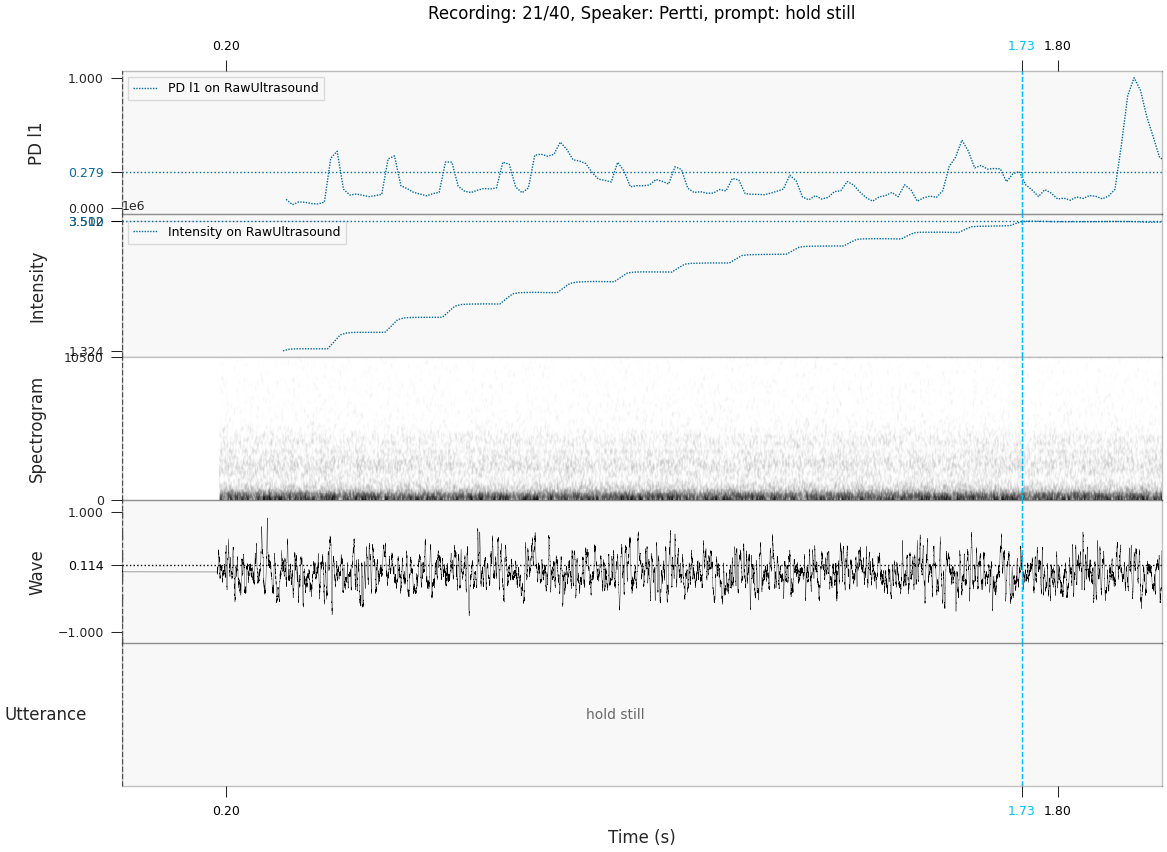
\includegraphics[width=\textwidth]{../figures/patkit_figure.png}
  % generated with
  \caption{Panels from top to bottom: Pixel Difference (PD), Image overall
  ultrasound intensity, Sound spectrogram, Sound waveform, and TextGrid
  (showing only the prompt 'hold still').}
    \label{fig:pd}
\end{figure}

\heading{Method and results.}
We demonstrate the effect with analysis of a technical
validation recording of the author. Figure~\ref{fig:pd} shows the analysis in
PATKIT \citep{PaloEtAl-PATKITPhoneticAnalysis-2026}.
As can be seen the image intensity ramps up by steps from beginning of the
ultrasound recording at about $t=0.3$~s to about $t=1.73$~s, at which point the
intensity plateaus. There is no speech in this recording as the speaker was
holding still. There is however a series of spikes in the PD curve (in addition
to natural twitching) which correspond to the moments when the intensity rises
a step. 
The effect on image quality can be seen in Figure~\ref{fig:ultrasound},
which shows the frame a the beginning of the recording and a frame at the end
of the intensity ramp. The latter image is brighter and has
potentially more detail.

\begin{figure}[!ht]
  \centering
  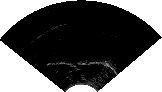
\includegraphics[width=.49\textwidth]{../figures/ultrasound_begin.png}
  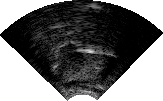
\includegraphics[width=.49\textwidth]{../figures/ultrasound_ramped_up.png}
  % generated with
  \caption{Ultrasound frames at the beginning of the recording (left) and at
  the end of the intensity ramp (right).}
    \label{fig:ultrasound}
\end{figure}

\heading{Conclusion.}
For new data the recommendation is simple: Plug the ultrasound machine into
mains power whenever possible and if you need to run it with only USB power,
make a note of that in your recording metadata and/or laboratory journal. For
old data, if you do not know that the device was plugged in to mains
electricity, there are two ways of checking if there is a problem with data
quality. First, play a recording and look at the data. If the ultrasound image
seems to get brighter they may be a problem. Second, examine the intensity
curves in PATKIT. You may need to look at more than one recording to see if
intensity is going up step-wise like in Figure~\ref{fig:pd}. In case the
intensity is ramping up, any intensity based measures might be unreliable.
Examining only PD curves in PATKIT or AAA
\citep{ArticulateInstruments-ArticulateAssistantAdvanced-2012-actual} is not
reliable as out of 40 test recordings made during the technical testing, only
two clearly showed a PD spike artefact pattern seen in Figure~\ref{fig:pd}. Not
seeing the pattern in the PD curve of a recording should not be taken as
evidence of the absence of the problem in a dataset, nor even the recording in
question, as it may affect event timing without being easily detectable. 

\setlength{\leftmargin}{1.5em}%
\setlength{\itemindent}{-1.5em}%
\setlength{\parsep}{0pt}%
\setlength{\itemsep}{0.2em}%

\heading{References.}
\vspace{-1.2em}
\renewcommand{\bibsection}{}
\renewcommand{\doiprefix}{}
\bibliographystyle{apacite}
\bibliography{science_combined,addendum}

% \kommentti{fix 'unpublished'}

% Custom environment for hanging indentation references
% \newenvironment{reflist}{%
%   \begin{list}{}{%
%     \setlength{\leftmargin}{1.5em}%
%     \setlength{\itemindent}{-1.5em}%
%     \setlength{\parsep}{0pt}%
%     \setlength{\itemsep}{0.2em}%
%   }
% }{%
%   \end{list}
% }
% \begin{reflist}
% \item Author, A. A. (2026). Title of reference. \textit{Journal Name}, Volume, Page range.
% \item Use a consistent format for references and inline citations.
% \end{reflist}

\end{document}
